\documentclass[landscape]{article}
\renewcommand{\abstractname}{}%去掉摘要头上的标题
\usepackage{xeCJK}
\usepackage[margin=2cm]{geometry}%调整页边距
\usepackage{graphicx}%插入图片
\usepackage{amsmath,bm}%数学公式宏包
\usepackage{amssymb}%特殊数学符号
\usepackage{caption}%图片标题处理
\usepackage{float}%处理图表浮动插入
\usepackage[section]{placeins}%防止图表浮动跨过section
\usepackage{subfigure}%插入多图时用子图显示的宏包
\usepackage{flushend,cuted}
\usepackage{makecell}
\usepackage{multirow}
\usepackage{amsmath}
\usepackage{rotfloat}
\usepackage{color}
\usepackage{xcolor}
\usepackage{longtable}
\usepackage{multicol}
\usepackage{enumitem}
\usepackage{geometry}
\usepackage{titlesec}

% \linespread{0.01}%全局行距
\pagestyle{empty}
\everymath{\displaystyle}
% \geometry{a4paper,left=0cm,right=0cm,top=0.1cm,bottom=0.5cm}
% \newcommand{\setParDis}{\setlength {\parskip} {0.1cm} }
% \newcommand{\setParDef}{\setlength {\parskip} {0pt} }
% \titleformat{\section}{\color{green}\footnotesize\bfseries}{\thesection}{.01em}{}
% \titleformat{\subsection}{\scriptsize\bfseries}{\thesubsection}{.01em}{}
% \titleformat{\subsubsection}{\tiny\bfseries}{\thesubsubsection}{.01em}{}


\begin{document}
\tiny
\begin{multicols}{3}

    \section{核物理实验方法期末开卷考试答案}
    ...
 
    1. 带电粒子的电离能量损失率($- \mathrm{d}E / \mathrm{d}x$)与入射带电粒子的质量关系为无关,与入射带电粒子的带电数 $z$ 的关系为 $z^2$ 。

    

    2. 在 $1 \ \mathrm{MeV}$ - $1000 \ \mathrm{MeV}$ 能量范围内,$\alpha$ 粒子的 $- \mathrm{d}E / \mathrm{d}x$ 随着能量的增加而减小(填增加或减小)。

    

    3. 重带电粒子的能量损失主要通过电离和激发, 在 $1 \ \mathrm{MeV}$ 以上电离为主;电子的能损主要通过电离和韧致辐射,随着能量的增加韧致辐射的贡献所占比例变大。

    

    4. Gaussian 分布的 FWHM 与 $\sigma$ 的关系式为$ \mathrm{FWHM} = 2.35 \sigma$ ,测量值 $x \pm \sigma$ 意味着真值落在 $x - \sigma$ 和 $x + \sigma$ 之间的几率为 $68\%$ 。

    

    5. 按衰减时间 (decay time) 由小到大的顺序排序 $\mathrm{NaI}$ ,$\mathrm{BaF_2}$ ,plastic :$\mathrm{BaF_2} (\mathrm{fast}) < \mathrm{plastic} < \mathrm{NaI} < \mathrm{BaF_2} (\mathrm{slow})$ 。

    

    6. 硅探测器和塑料闪烁体探测器都是 $\beta$ 射线探测中常见的探测器。对于能量测量和活度测量应优先使用哪种探测器?为什么?

    答:对于能量测量应该优先使用硅探测器,对于活度测量应优先使用塑料闪烁体探测器。

    原因:硅探测器产生电子-空穴对所需的能量很小,具有卓越的能量分辨率。密度相对较大,具有更好的阻止本领,阻停同样能量的束流,所需要的体积较小,更紧凑。塑料闪烁体探测器的能量分辨率较差,但是衰减时间仅几个纳秒,上升时间约 $4$ 纳秒(硅探测器的上升时间约 $60 \ \mathrm{ns}$),具有极好的时间分辨率,适宜做时间测量。

    

    7. 能量为 $2 \ \mathrm{MeV}$ 的单能 $\gamma$ 光子被 $\mathrm{NaI} + \mathrm{PMT}$ 探测器所探测。

    \begin{itemize}
    \item 画出能谱($\mathrm{d}N / \mathrm{d}E \sim E $),标注主要特征。
            \begin{figure}[H]
                \centering
                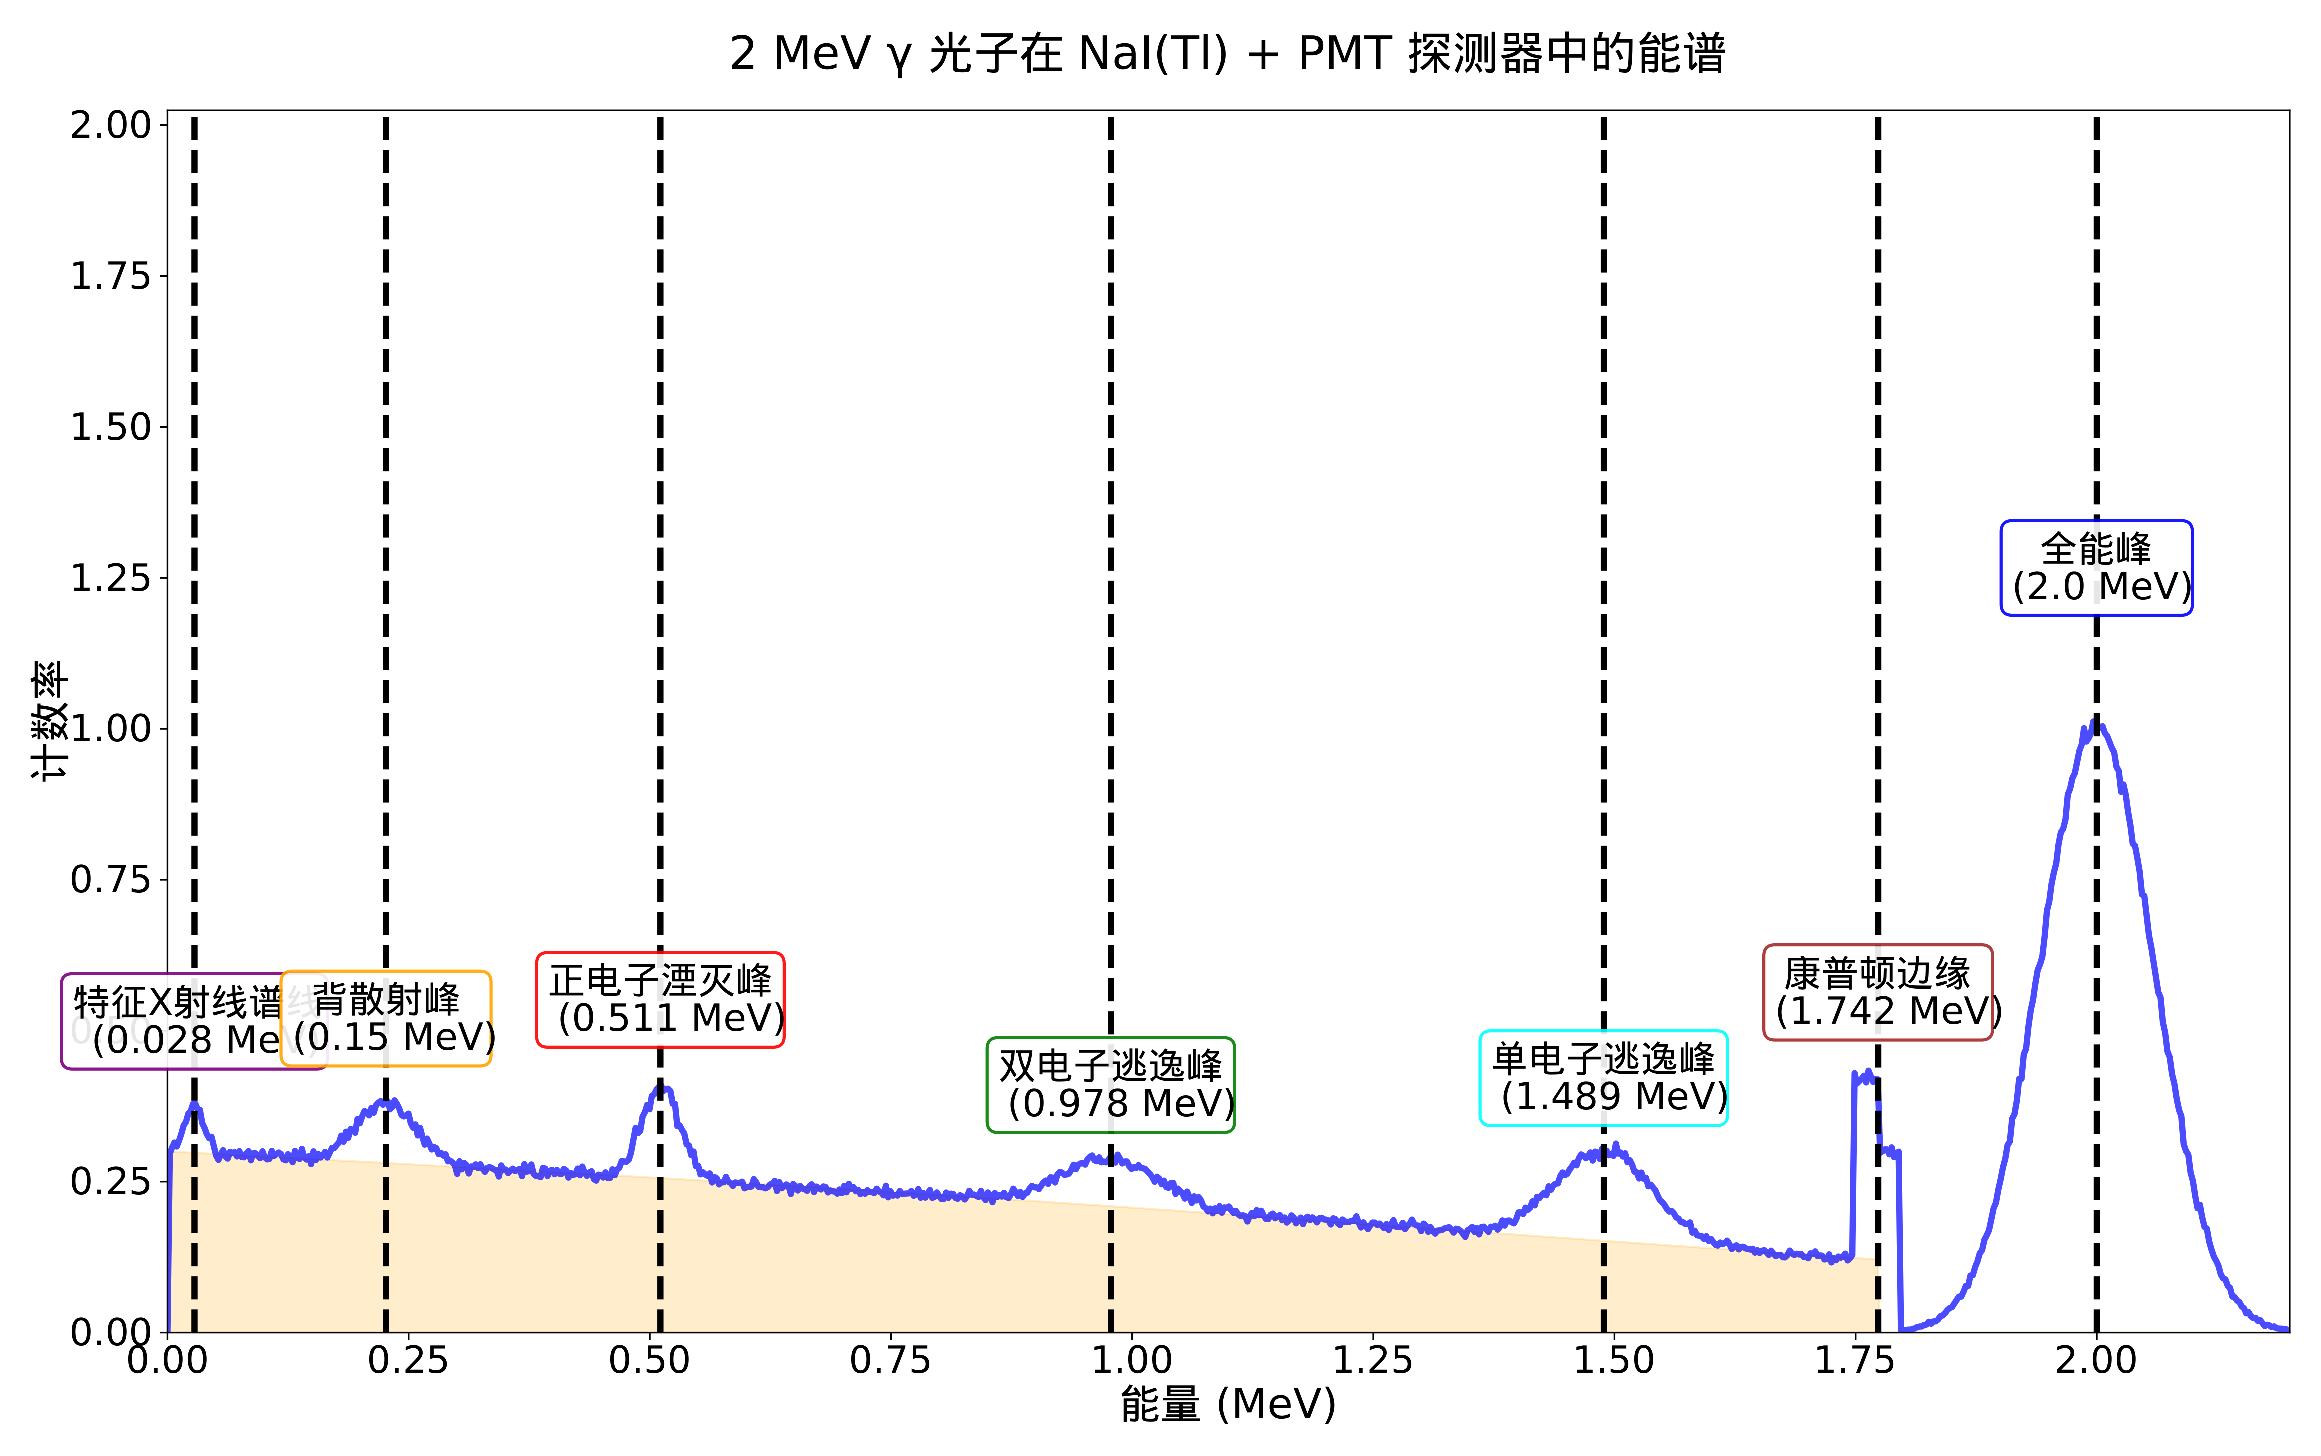
\includegraphics[scale=0.15]{NaI_gamma_spectrum.eps}
                \label{fig:gamma_spectrum}
            \end{figure}
    \item 简述谱中各特征的产生机制。
            第一个峰是特征 X 射线谱线,第二个是由于背散射导致的峰,第三个是正电子湮灭导致的峰,第四个是全能峰的双电子逃逸峰,第五个是单电子逃逸峰,第六个是康普顿边缘,最后一个是全能峰。

        全能峰(Full-energy peak)  

            位置:  
        \begin{equation}
        E = X
        \end{equation}

            来源: $\gamma$ 光子在晶体中完全沉积其能量(光电效应 / 多次康普顿散射后再经光电效应)。  

        康普顿连续谱以及康普顿边缘(Compton edge)  

            康普顿边缘位置:  
        \begin{equation}
        E_\mathrm{C} = X\left(1 - \frac{1}{1 + 2X / m_e c^2}\right)
        \end{equation}

            来源: 单次康普顿散射中,反冲电子获得的最大动能所对应的能量端点。  

        背散射峰(Backscatter peak)  

            位置:
        \begin{equation}
        E_\mathrm{B} = \frac{X}{1 + 2X / m_e c^2}= \frac{X}{1 + \frac{m_e c^2}{2X}}
        \end{equation}

            来源: $\gamma$ 光子在探测器外部发生 $180 $ 康普顿散射后,再返回并在晶体中被吸收。  

        正电子湮灭峰($511\ \mathrm{keV}$)  

            位置:  
        \begin{equation}
        E = 0.511 \ \mathrm{MeV}
        \end{equation}

            来源: 当 $X > 1.022 \ \mathrm{MeV}$ 时发生对产生,正电子与电子湮灭产生两条 $511 \ \mathrm{keV}$ 光子。  

        单电子逃逸峰(Single escape peak)  

            位置:  
        \begin{equation}
        E = X - 0.511 \ \mathrm{MeV}
        \end{equation}

            来源: 对产生后,两条湮灭光子中有一条逃逸出探测器。  

        双电子逃逸峰(Double escape peak)  

            位置:  
        \begin{equation}
        E = X - 1.022 \ \mathrm{MeV}
        \end{equation}

            来源: 对产生后,两条 $511 \ \mathrm{keV}$ 湮灭光子全部逃逸出探测器。  

        特征 X 射线峰(Characteristic X-rays)  

            来源核素: $\mathrm{NaI}$ 探测器中主要来自 $\mathrm{I}$(碘)原子的 K 线。  

            典型能量位置:  
        \begin{equation}
        28 \sim 33 \ \mathrm{keV}
        \end{equation}

            来源: $\gamma$ 光子发生光电效应后,原子内壳层空穴退激辐射产生的特征 X 射线。

    \item 如果探测器的灵敏体积由小到大发生变化,能谱将发生什么变化?

    灵敏体积变大,探测效率增加,被探测到的 $\gamma$ 射线沉积的能量也增多。全能峰面积和多重康普顿散射增加,其他峰位包括康普顿坪减小。等探测器的灵敏体积“无限大”时,只剩下全能峰。
    \item 描述课上讲过的 $\gamma$ 能谱测量中降低康普顿连续谱对低能区影响的两种方法。

        - 使用反康普顿谱仪:如果半导体探测器和包裹在半导体探测器外侧的 BGO 探测器同时有信号输出,则可以利用反符合的方式,拒绝在半导体中产生的信号,这样最后半导体探测器输出的信号就只有全能峰的信号。( BGO 探测效率大);

        - 使用复合锗探测器:设置多块锗探测器,若某一 $\gamma$ 先后在多个小探测器中沉积能量产生信号,则可通过符合的方式把多个探测器的输出信号幅度相加,以此增加最后能谱的峰康比。
    \end{itemize}

    8. 从电路负载和阻抗匹配对信号影响的角度,描述能量路和时间路电子学的前后级的 $Z_{\mathrm{out1}}$ 和 $Z_{\mathrm{in2}}$ 之间满足什么条件,为什么?

    答:
    能量测量:$Z_{\mathrm{in1}} = 1000 \ \Omega$ ,$Z_{\mathrm{out2}} < 1 \ \Omega$ ;时间测量:$Z_{\mathrm{in1}} = 50 \ \Omega$ ,$Z_{\mathrm{out2}} = 50 \ \Omega$ 。

    原因:
    用于能量测量、慢信号时最好总是有 $Z_{\mathrm{out2}} \ll Z_{\mathrm{in1}}$ ,这样当负载连接时,信号电平就不会改变。
    用于时间测量、快速信号时它要求有 $Z_{\mathrm{out2}} = Z_{\mathrm{in1}}$ ,这就是射频电路的情况,以避免信号反射。

    

    9. 用金硅面垒探测器测 ${}^{210}\mathrm{Po}$ 的 $\alpha$ 粒子能谱。
    \begin{itemize}
        \item 逐步增加反偏电压时观测到的脉冲幅度和分辨率有何变化,原因是什么?

        加反偏电压会使金硅面垒探测器的灵敏区增加,进而使得探测器中沉积的能量增大直至达到最大值饱和不变,因此脉冲幅度会先增加然后不变;对于分辨率而言,相对分辨率反比于沉积能量的 $1/2$ 次方,随着沉积能量的增大,能量分辨率逐渐提高,直至不变。

        \item 描述利用 $\alpha$ 放射源确定探测器工作偏压的方法?

        1.  选择适当的 $\alpha$ 放射源:选择一个放射性核素,通常是一个放射性的 $\alpha$ 粒子源。

        2.  放置 $\alpha$ 放射源:将 $\alpha$ 放射源放置在离探测器表面一定距离的位置,以确保探测器可以被辐射到。

        3.  逐步调整工作偏压:从零开始逐步增加探测器的工作偏压,监测探测器输出的信号。

        4.  记录信号变化:随着工作偏压的增加,记录 $\alpha$ 粒子探测信号的变化。

        5.  确定最佳工作偏压:当输出信号的峰不再改变时,确定了最佳工作偏压。
    \end{itemize}

    10. 写出望远镜法、脉冲形状甄别法进行粒子鉴别的原理?

        答:

        脉冲波形法:入射粒子的 $\mathrm{d}E / \mathrm{d}x$ 的值越大,闪烁光里面的慢成分越多。在实验中,入射粒子在探测器中产生信号的尾部面积与脉冲总面积的比值越大,则说明粒子的 $\mathrm{d}E / \mathrm{d}x$ 越大,因此可以通过辨别脉冲形状来鉴别粒子。

        望远镜法:将两块探测器联合在一起,其中第一块探测能量损失,第二块探测粒子的能量。根据电离能损公式:$\mathrm{d}E/\mathrm{d}x \propto A Z^{2}/E$,当第一块探测器厚度很薄时,粒子的沉积能量很小,可以认为粒子在第一块探测器中的能量为一常数,因此粒子在第一块探测中的沉积能量 $\Delta E \propto A Z^{2}/E$,再利用第二块探测器探测粒子能量,将两块探测器的测量值绘制在一个图中,由于入射粒子的质量数以及质子数不同,可以得到一系列曲线,通过这些曲线可以辨别粒子。

        

    11. 简述带电粒子在电离室区和正比区发生的物理过程。写出在本课程中出现的几种气体探测器的名称,至少 $5$ 种,并指明工作在哪一区。

    答:

    电离室区:随着外加电压增大,离子漂移速度增加,电子吸附、扩散效应的影响减小,发生复合的机会减小,被收集的电荷数增加。电压达到一定值($V_a$)时,基本不存在复合,总电离数($N_0$)全部被电极收集,达到饱和。在一定电压范围内($ V_a - V_b$),被收集电荷不再增加,达到饱和。

    正比区:工作电压大于 $V_b$ 后,外加电场很强,电离电子在漂移过程中获得的能量很大,使气体分子再电离,又产生次级离子对。次级电子在漂移时又可能加速到足以再次产生次级离子对。如此不断继续下去,使电离的离子对数目比原总电离对数目 $N_0$ 增加很多,称为气体放大。经气体放大得到的电荷数 $N$ 与原总电离数 $N_0$ 之比,叫做气体放大倍数 $M$ , $M = N / N_0$ ,气体放大倍数随电压的增加而增加。对确定的探测器,外加电压一定时,放大倍数一定。

    几种气体探测器及其工作区:

    1.  电离室(电离室区);

    2.  正比计数器(正比区);

    3.  多丝正比室(正比区);

    4.  PPAC(正比区);

    5.  G-M 计数器(G-M区)。

        
    12. 试用误差传递公式求出飞行时间法 (TOF) 测量中子能量 $E_n$ 的相对误差 (不考虑 start 探测器时间分辨),并讨论减少测量误差的方法。

    符号:飞行距离 $L$ ,飞行时间 $\mathrm{TOF}$ ,stop 探测器厚度 $\sigma_{L}$ ,stop 探测器时间分辨 $\sigma_{t}$ 。

    答:

    首先有:
    \begin{equation}
    E_n = \frac{m_nL^2}{2\mathrm{TOF}^2}.
    \end{equation}

    已知有距离的不确定度 $\sigma_{L}$ 以及飞行时间的不确定度 $\sigma_{\mathrm{TOF}}$ 。根据不确定度传递公式,有
    \begin{equation}
    \sigma_{E_n}^2 = (\partial_LE_n)^2\sigma_{L}^2 + (\partial_\mathrm{TOF}E_n)^2\sigma_{\mathrm{TOF}}^2 + 2\partial^2_{L,\mathrm{TOF}}E_n \mathrm{cov}(L,\mathrm{TOF}),
    \end{equation}
    即
    \begin{equation}
    \sigma_{E_n}^2 = \left(\frac{m_nL}{\mathrm{TOF}^2}\right)^2\sigma_{L}^2 + 
    \left(\frac{m_nL^2}{\mathrm{TOF}^3}\right)^2\sigma_{\mathrm{TOF}}^2 -2 
    \frac{m_n^2L^3}{\mathrm{TOF}^5} \mathrm{cov}(L,\mathrm{TOF}).
    \end{equation}

    于是相对误差可以写为
    \begin{equation}
        \begin{aligned}
            R &= \frac{\sqrt{\left(\frac{m_nL}{\mathrm{TOF}^2}\right)^2\sigma_{L}^2 + \left(\frac{m_nL^2}{\mathrm{TOF}^3}\right)^2\sigma_{\mathrm{TOF}}^2 -2\frac{m_n^2L^3}{\mathrm{TOF}^5}\mathrm{cov}(L,\mathrm{TOF})}}{E_n}\\ &= \frac{2}{L}\sqrt{\sigma_L^2 +\frac{L^2}{t^2}\sigma_t^2 - 2\frac{L}{t}\mathrm{cov}(L,\mathrm{TOF})}.
        \end{aligned}
    \end{equation}
    一般认为 $\mathrm{cov}(L,\mathrm{TOF}) = 0$ 。

    减小误差的方法:

    \begin{itemize}
        \item 增加飞行距离 $L$ 或者飞行时间 $\mathrm{TOF}$ ;
        \item  选用密度大的阻止探测器以减小 $\sigma_{L}$ ;
        \item  选用时间分辨小的 stop 探测器以减小 $\sigma_{t}$ 。
    \end{itemize}
        

    13. 简述前置放大器和主放大器的功能。

        答:
        大多数核探测器输出的信号幅度很小,如硅探测器,直接输出信号小于 $1 \ \mathrm{mV}$ 。幅度小的信号在传输过程中易受到噪声的干扰,不利于远距离传输。因此,信号在传输前,需要先进行放大处理。

        前置放大器:位于探测器和下一级电子学之间。将探测器的输出信号进行放大,提高信噪比;提供阻抗匹配;对信号脉冲进行整形,方便后续的信号处理。
            
        前置放大器的分类:电压灵敏型;电荷灵敏型(主要);电流灵敏型。
            
        主放大器:又叫整形放大器,位于前置放大器后,由 CR 微分电路和 RC 积分电路构成,将前放的输出信号整成准高斯型。经过谱仪放大输出器输出的信号顶端平,有利于后面的幅度分析;放大和成形,改善信噪比。

        

    14. 简述前沿甄别和恒比定时甄别的定时原理及适用范围。

        答:

        前沿定时法:
            原理:当输入信号超过一个固定的阈值水平时,它会产生一个逻辑脉冲,该阈值水平应该高于噪声水平,以防止对噪声信号的杂散触发。
            适用范围:用于输入脉冲幅度和波形变化不大的情况。

        恒比定时法(CFD):
            原理:将输入信号 $Af(t)$ 进行翻转延时 $-Af(t-\tau)$ 以及缩小处理 $rAf(t)$ 。\textbf{注意延时时间 $\tau$ 要大于信号的上升时间}。当翻转延时的信号幅度与缩小处理的信号幅度之和为零时($rAf(t)-Af(t-\tau) = 0$),输出信号。
            主要用于上升时间不变的(保证延迟时间固定)快响应探测器,如有机闪烁体探测器。如果所有信号的上升时间 $t_r$ 相同,则触发时间与信号最大值无关,应该选用 CFD 。

        补充:幅度与上升时间补偿定时(ARC)
            此时要求\textbf{延时时间 $\tau$ 要小于信号的上升时间},其余结论类似 CFD 。ARC 主要适用于上升时间变化的信号触发。但是实际性能不如 CFD ,因为相减之后的表达式斜率比较小,受噪声影响大。


    15. 用两个 HPGe 探测器来测量活度为 $n_0$ 的 ${}^{60}\mathrm{Co}$ 放射源的一对 $\gamma$ 光子,探测器探测效率分别为 $\varepsilon_1$ 、$\varepsilon_2$ ,两个探测器时间信号的宽度均为 $\tau$ 。

    \begin{itemize}
        \item 画出符合法测量 ${}^{60}\mathrm{Co}$ 的两个 $\gamma$ 是否有级联关系的电路框图(包含前置放大器、分路器、时间甄别、Delay、符合单元、触发器、ADC、TDC、ADC gate、TDC start)。
        
        答:符合电路(题目可能不一样)

        \begin{figure}[H]
            \centering
            \includegraphics[scale=0.15]{kuangtu1.jpg}
            \label{fig:kuangtu1}
        \end{figure}

        \item 给出用符合法测得的真符合和偶然符合的计数率。
        
        假设探测器 $1$ 记录 $\gamma_1$ 光子,对放射源立体角为 $\Omega_{\gamma_1}$ ;假设探测器 $2$ 记录 $\gamma_2$ 光子,对放射源立体角为 $\Omega_{\gamma_2}$ 。

        第一道计数率为:
        \begin{equation}
        n_{\gamma_1} = n_0 \Omega_{\gamma_1} \varepsilon_{\gamma_1},
        \end{equation}
        第二道计数率为:
        \begin{equation}
        n_{\gamma_2} = n_0 \Omega_{\gamma_2} \varepsilon_{\gamma_2},
        \end{equation}
        真符合计数率为:
        \begin{equation}
        n_{\mathrm{tc}} = n_0 \Omega_{\gamma_1} \varepsilon_{\gamma_1} \Omega_{\gamma_2} \varepsilon_{\gamma_2}.
        \end{equation}
        偶然符合计数率为:
        \begin{equation}
        n_{\mathrm{rc}} = 2 \tau n_0^2 \Omega_{\gamma_1} \varepsilon_{\gamma_1} \Omega_{\gamma_2} \varepsilon_{\gamma_2}.
        \end{equation}
        真偶符合比为:
        \begin{equation}
        \frac{n_{\mathrm{tc}}}{n_{\mathrm{rc}}} = \frac{1}{2 \tau n_0}.
        \end{equation}
    \end{itemize}        

    \section{课堂中提到的重点}
    
    \subsection{测量 PN 结怎么加压才是正偏和反偏}

    用万用表的红黑笔分别反向夹住 PN 结测量,哪边电阻高就哪边是反偏。这种测量方法需要在避光条件下测量,否则光激发会导致不论怎么测电压都差不多。

    \subsection{如何判断是不是完全耗尽}

    用单能放射源从两个方向照射,例如下图

    \begin{figure}[H]
        \centering
        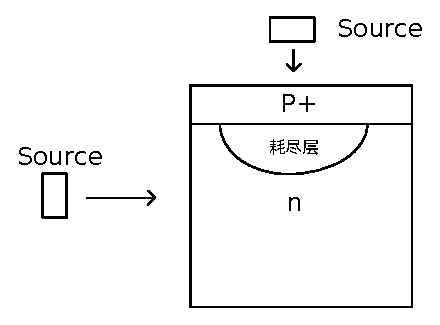
\includegraphics[scale=0.45]{wha.eps}
    \end{figure}

    然后可以测到幅值-电压曲线,如下图

    \begin{figure}[H]
        \centering
        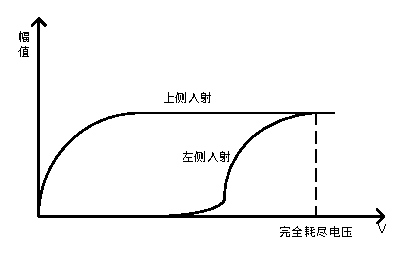
\includegraphics[scale=0.45]{wha1.eps}
    \end{figure}

    这样子就可以确定完全耗尽电压。
    
    \section{主要内容笔记}
    \subsection{Bethe - Bloch 公式}
    \begin{equation}
        \begin{aligned}
            \frac{\mathrm{d}E}{\mathrm{d}x} = &\underbrace{\frac{2\pi k^2 e^4 N_A}{m_e c^2 \beta^2}}_{\text{常数因子}} \underbrace{\frac{z^2}{\beta^2}}_\text{入射粒子}\underbrace{\frac{\rho Z}{A}}_{\text{吸收体}}
            \left[ 
            \ln\left(\frac{2m_e c^2 \beta^2 \gamma^2 T_{\text{max}}}{I^2}\right)\right. \\
            &\left. - \underbrace{2\beta^2}_{\text{相对论修正}} 
            - \underbrace{\delta}_{\text{密度效应}} 
            - \underbrace{2\frac{C}{Z}}_{\text{壳修正}} 
            \right]
        \end{aligned}
    \end{equation}
    其中密度项 $\delta$ 在高能区很重要;壳修正在低能区很重要。
    \begin{itemize}
        \item 低能区: $\mathrm{d}E / \mathrm{d}x \propto v^{-2}$ ;
        \item 高能区: $\mathrm{d}E / \mathrm{d}x \propto \ln{v^2}$;
        \item 与原子序数与核子数的关系:$\mathrm{d}E / \mathrm{d}x \propto \rho Z/A$。
    \end{itemize}

    Bethe - Bloch 公式在低能情况下失效,总的阻止能力与能量的关系如下图所示。

    \begin{figure}[H]
        \centering
        \includegraphics[scale=0.25]{1.png}
    \end{figure}

    \subsection{误差传递公式}
    \begin{equation}
        \sigma_a^2 = \left.\left(\frac{\partial f}{\partial x}\right)^2\right|_{(\bar x,\bar y)}\sigma_x^2 + \left.\left(\frac{\partial f}{\partial y}\right)^2\right|_{\sim}\sigma_y^2 + \left.2\frac{\partial f}{\partial x} \frac{\partial f}{\partial y}\right|_{\sim} \mathrm{cov}(x,y).
    \end{equation}


    \subsection{探测器}

    \begin{itemize}
    \item 气泡室——过饱和液体
    \item 核乳胶,位置分辨能力最好的
    \end{itemize}

    \subsection{框图补充}
    \begin{itemize}
        \item 测量锗探测器(特别是大体积HPGe探测器)的时间分辨率
                \begin{figure}[H]
                    \centering
                    \includegraphics[scale=0.25]{2.png}
                \end{figure}
    \end{itemize}

    \subsection{采样与数字化}
    ...

    一个连续信号采样之后,其频谱变成了离散的频谱,离散频谱中会有原始频谱的镜像,如果采样频率不够高,镜像频谱会和原始频谱重合,导致混叠失真。

    保证足够高的采样频率可以避免混叠失真,如果有一个理想的低通滤波器,只需要采样频率应该是信号最高频率的两倍就可以完全分离镜像频谱和原始频谱;但是由于实际滤波器不可能直接就是一个阶梯,实际采样频率需要高于信号最高频率的两倍。

    一个常用的采样器是 Flash ADC ,具体结构如下

    \begin{figure}[H]
        \centering
        \includegraphics[scale=0.2]{4.png}
    \end{figure}

    它能实现 $0.2 \ \mathrm{ns}$ 采样时间。在采样时刻,输入电压 $V_i$ 被锁定;它同时与一组等间隔参考电压比较;比较器输出温度计码;编码器将其转换为数字输出;由于电压只能落在有限区间内,量化误差不可避免。


    实际的连续信号经过采样以及数字化后被储存,其中数字化会给信号引入一个均匀分布的随机噪声。

    \begin{figure}[H]
        \centering
        \includegraphics[scale=0.2]{3.png}
    \end{figure}

    数字化

    
\end{multicols}
\end{document}